\documentclass[a4paper, 12 pt]{report}
\usepackage{multirow}
\usepackage{graphicx}
\usepackage{tabularx}
\usepackage{geometry}
\geometry{left=2.5cm,right=2.5cm,top=2.5cm,bottom=2.5cm}
\usepackage{algorithm}  

% -------------------------------------------------------------------------------------
% BEGIN DOCUMENT
% -------------------------------------------------------------------------------------
\begin{document}
\title{Drone User Manual}
\author{Shao Hui z5155945}
\date{}
\maketitle
\pagestyle{empty}
\setcounter{section}{0}
% -------------------------------------------------------------------------------------
% TABLE OF CONTENTS
% -------------------------------------------------------------------------------------
\tableofcontents
\newpage

% -------------------------------------------------------------------------------------
% INTRODUCTION
% -------------------------------------------------------------------------------------
\section{Introduction}
This project simulates a drone searching a certain mountain for accident scene.\\
Drone can search a mountain of 64m$\times$64m with max height of 64m and minimal height of 0m.
This mountain is represented by a 64$\times$64 matrix. This project provide some tools to randomly generate such mountain which will be discussed in section 3.\\
This project uses two press key, and a 4$\times$4 keypad to control simulation. The simulate process will be discussed in section 4.\\
The mountain view is showed as follow.\\
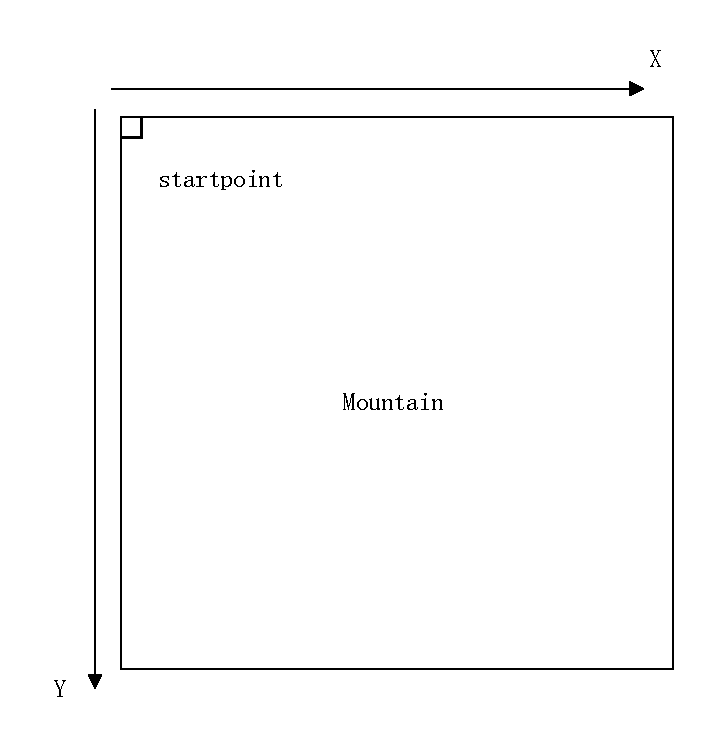
\includegraphics[height = 130mm]{mountain_diagram.pdf}
\newpage

% -------------------------------------------------------------------------------------
% DAEMONS
% -------------------------------------------------------------------------------------
\section{Board Connection}
\begin{table}[!htbp]
\resizebox{\textwidth}{!}{
\begin{tabularx}{13cm}{XXXX}
\multicolumn{2}{l}{AVR Pins (top and bottom row)}
     & \multicolumn{2}{l}{Input/Output Device Pins (middle row)}\\\hline
    Port Group & Pin & Port Group & Pin\\\hline
    PORT A & PA4 & LCD CTRL & BE\\
    PORT A & PA5 &LCD CTRL & RW\\
    PORT A & PA6 &LCD CTRL & E\\
    PORT A & PA7 & LCD CTRL& RS\\\hline
    PORT C & PC0 & LED BAR & LED2\\
    PORT C & PC1 & LED BAR & LED3\\
    PORT C & PC2 & LED BAR & LED4\\
    PORT C & PC3 & LED BAR & LED5\\
    PORT C & PC4 & LED  BAR & LED6\\
    PORT C & PC5 & LED BAR & LED7\\
    PORT C & PC6 & LED BAR & LED8\\
    PORT C & PC7 & LED BAR & LED9\\\hline
    PORT D & RDX4 & INPUTS & PB0\\
    PORT D & RDX3 & INPUTS & PB1\\\hline
    PORT F & PF0 & LCD DATA & D0\\
    PORT F & PF1 & LCD DATA & D1\\
    PORT F & PF2 & LCD DATA & D2\\
    PORT F & PF3 & LCD DATA & D3\\
    PORT F & PF4 & LCD DATA & D4\\
    PORT F & PF5 & LCD DATA & D5\\
    PORT F & PF6 & LCD DATA & D6\\
    PORT F & PF7 & LCD DATA & D7\\
    PORT F & PF8 & LCD DATA & D8\\\hline
    PORT L & PL0 & KEYPAD & C3\\
    PORT L & PL1 & KEYPAD & C2\\
    PORT L & PL2 & KEYPAD & C1\\
    PORT L & PL3 & KEYPAD & C0\\
    PORT L & PL4 & KEYPAD & R3\\
    PORT L & PL5 & KEYPAD & R2\\
    PORT L & PL6 & KEYPAD & R1\\
    PORT L & PL7 & KEYPAD & R0\\\hline
    PORT E & PE3 & JP92 & RIGHT\\\hline
    MOTOR & Mot & JP91 & RIGHT
\end{tabularx}
}
\end{table}
JP92 and JP91 isolate POT and let it be connected between pwm generator and motor to make sure the motor wont crash the board. 
\newpage

% -------------------------------------------------------------------------------------
% Mountain Generator
% -------------------------------------------------------------------------------------
\section{Mountain Generator}
This project provided a random mountain generator written in python called generator.py that will generate a 64$\times$64 matrix and write it to the "mountain.asm" file which will be included into the source code.\\\\
This generator uses such technique,\\
1. Randomly generate a peak in position x, y with height h.\\
2. Generate down from the peak to its neighbour grid until height became less then 10.\\
3. Combine this graph with the former mountain map and cut out the positions that are lower than the former map.\\
4. Repeat this procedure for several times.\\\\
This technique always generate a mountain that make sense. You can also use your own generator or simply type in a mountain that suits your need. But make sure when you assemble the project, label your mountain with a label "mountain".
\newpage
% -------------------------------------------------------------------------------------
% Control Procedure
% -------------------------------------------------------------------------------------
\section{Control Procedure}
Every time when the board is reset. The LCD will display a string "Input X:".\\
You should always follow such emulate procedure.\\
1. Input some number within 64 using keypad end with "\#", which is the row number of the accident scene. If your input is invalid, led will flash three times and loop until valid number is input.\\
2. After LCD showed "Input Y:", input some number within 64 using keypad end with "\#", which is the column number of the accident scene. If your input is invalid, led will flash three times and loop until valid number is input.\\
- If x and y are both less than 64, the accident can be found. If one of them are set to 64, the accident scene can not be found.\\
3. After LCD showed "READY", press PB0 to start search. LED will flash 3 times to indicate the start of search. LCD will show drone's current position and flying direction.\\
Motor will be spinning.\\
4. Once the drone get to each grid, LCD will show it is searching, and the motor should spin at low speed to indicate it is suspending.\\
5. During search, you can always press PB1 to abort the search. Drone will immediately fly back to position (0,0). LCD will show "ABORT".\\
6. After finding the accident scene. Drone will immediately fly back to position (0,0).
LCD will show "FOUND" and the position of the accident scene. Motor will stop. If a accident scene not fount, LCD will show "NOT FOUND", and motor also stop.
\end{document}
